% 以下の3行は変更しないこと.
\documentclass[T]{compsoft}
\taikai{2014}
\pagestyle {empty}

\usepackage [dvipdfmx] {graphicx}

% ユーザが定義したマクロなどはここに置く.ただし学会誌のスタイルの
% 再定義は原則として避けること.
\usepackage{proof,amsmath,bcprules,listings,lstcoq,jlisting,enumitem,url,amsthm,nccmath,subfig}
\usepackage{mymacros}


\begin{document}

% 論文のタイトル
\title{\api の Coq による形式化}

% 著者
% 和文論文の場合,姓と名の間には半角スペースを入れ,
% 複数の著者の間は全角スペースで区切る
%
\author{安武 祥平
%
% ここにタイトル英訳 (英文の場合は和訳) を書く.
%
\ejtitle{A formalization of \apie using Coq}
%
% ここに著者英文表記 (英文の場合は和文表記) および
% 所属 (和文および英文) を書く.
% 複数著者の所属はまとめてよい.
%
\shozoku{Shohei Yasutake}{東京工業大学大学院情報理工学研究科計算工学専攻}%
{Dept.\ of Computer Science, Tokyo Institute of Technology}}

% 和文アブストラクト
\Jabstract{%
  アクターモデルは並行計算のモデルのひとつであり,アクターと呼ばれる計算主体がそれぞれ並列に動作し互いに非同期にメッセージを送りあって計算を進める.
  アクターモデルは,アクターの名前は一意であるという性質,他のアクターの名前あるいはメッセージとして送られてきた名前ではアクターを作れないという性質,アクターにはいつでもメッセージを送ることができるという性質,の3つの性質を持っている.
  これらの性質を満たすように $\pi$ 計算に型を付け,アクターモデルとしての振る舞いを強制させたものに \api があるが,\api が確かにアクターモデルとしての振る舞いを示すかどうかについて形式的な証明はまだ与えられていない.
  そこで,本研究では,\api およびその型システムの定義を,等価だが証明を進めやすい定義に変更するなどの工夫を行い,\api の型システムがアクターモデルとしての振る舞いを強制することについて,定理証明支援系 Coq を用いて形式的な証明を与えた.
}

% 英文アブストラクト(本サンプルの原論文にはなし)
\Eabstract{
英語アブスト
}
%
\maketitle \thispagestyle {empty}

\section{はじめに}

アクターモデル\cite{Agha:1986aa}は並行計算のモデルのひとつであり,互いに非同期メッセージをやりとりするアクターと呼ばれる計算主体(computing entity)によって計算システムを表現する.
現在,アクターモデルやその発展形である並行オブジェクト計算モデル\cite{Yonezawa:1986aa}にもとづく言語は多数提案・実装されてきており,それらの研究成果をもとに現在 Scala や Erlang, Akka 等,アクターモデルを並行計算の基盤としたプログラミング言語やライブラリが実用に供されている.
そのため,アクターモデルによって構成されたシステムの形式的検証は喫緊の課題であると考えられる.

形式的検証の研究に先立ち,アクターモデルの形式的意味論については古くから研究が行なわれてきた.
例えばClingerによるPowerdomainを用いた表示的意味\cite{Clinger:1981aa}や,Aghaによる操作的意味\cite{Agha:1986aa}とその発展\cite{Agha:1997aa}がある.
これらの研究では,公平性やいくつかの等価性についての成果があるものの,プロセス代数を元に発展してきた$\pi$計算等に比べると発展途上であると言わざるを得ない.

一方,形式的検証についてはアクターで記述されたシステムのモデル検査を可能にする
モデル記述言語Rebeca\cite{Sirjani:2011aa},証明支援系を含むプログラミング言語Athenaを用いた検証例\cite{Musser:2013aa},およびCoqを用いたアクターモデルの定式化と検証例\cite{Garnock-Jones:2014aa}など,最近になっていくつかの研究成果が出ている.
本研究はアクターで構成されたシステムのCoqによる形式的検証のための枠組みを提供することを目的としている.

アクターモデルのもつ性質には,アクターの名前は一意であるという性質(名前の一意性),メッセージとして送られてきた名前でアクターを作ることはできないという性質(名前の新鮮性),アクターにはいつでもメッセージを送ることができるという性質(アクターの永続性)が含まれる.
これらの性質をみたす項を構成するよう\(\pi\)計算に型システムを導入し,アクターモデルを形式化したA\(\pi\)計算がAghaらによって提案されている\cite{Agha:2004aa}.

\api の型システムにおける健全性とは,型付けされた項はアクターモデルとしての振る舞いを示すということであるが,その証明は形式的に与えられていない.
本研究では,A\(\pi\)計算およびその型システムの定義を見直すことで,型システムの健全性について定理証明支援系Coqを用いた形式的な証明を与える.また,本研究はA\(\pi\)計算自体の正しさの検証ということも目的としているため,A\(\pi\)計算の定義は等価なものへの変更でない限り変更しないものとする.
%% このようなアクターモデルの性質を満たすように設計された,$\pi$ 計算を用いた形式化として,\api が 提案されている[3] .
%% Aπ計算は,π計算に型を付けることによってアクターモデルの性質を表現することを目的としており,may-testingと呼ばれる,二つのアクターの等価性についての理論に使われている.
%% このような基礎的な理論には形式的な証明があることが望ましい.
%% しかし,Aπ計算の性質に対して形 式的な証明を与えているものはまだない.

%% 本研究では,Aπ計算の型付けにおける健全性に対して,形式的な証明を与えることを目的とする.
%% 形式的な証明を与えるためのツールとして定理証明支援系Coqを用いる.
%% また,Coqで証明する際に,Aπ計算およびその型システムについての定義をより具体的なものに定義しなおすことによって,より簡単に証明を行えるようにしている.



%%  $ \pi $ 計算やアクターモデルは並行計算のモデルとして発展してきた.アクターモデルはアクターと呼ばれる計算主体 (computing entity) が並列に動作し,互いに非同期にメッセージを送り合うことによって計算を行う.
%% アクターモデルの持つべき性質として,アクターの名前は一意であるという性質,メッセージとして送られてきた名前でアクターを作ることはできないという性質,アクターにはいつでもメッセージを送ることができるという性質,を持っている.

%% このようなアクターモデルの性質を満たすように設計された,$\pi$ 計算を用いた形式化として,\api が提案されている\cite[Dean2008]{Agha:2004aa} .\api は,$\pi$ 計算に型を付けることによってアクターモデルの性質を表現することを目的としており,May Testing と呼ばれる,二つのアクターの等価性についての理論に使われている.


%% このような基礎的な理論には形式的な証明があることが望ましい.しかし,\api の性質に対して形式的な証明を与えているものはまだない.


%% \subsection{目的}

%% 本研究では,\api の型付けにおける健全性に対して,形式的な証明を与えることを目的とする.
%% 形式的な証明を与えるためのツールとして定理証明支援系 Coq を用いる.
%% また,Coq で証明する際に,\api およびその型システムについての定義をより具体的なものに定義しなおすことによって,より簡単に証明を行えるようにしている.


%% \subsection{構成}

%% 第2章でアクターモデルや $\pi$ 計算,定理証明支援系 Coq などの背景知識を述べる.
%% 第3章で \api について説明し,第4章では \api およびその型付けについて定理証明支援系 Coq 上で定義し,その健全性の証明方針を述べる.第5章ではまとめとして,結論と今後の課題を述べる.


%% 自己調整二分木(スプレー木, splay tree) \cite{ST85}は,アクセスした節
%% 点に対して扁平化(splaying)操作(\ref{subsection:splaying}節)
%% を施すことにより,木の形状を動的に最適化す
%% る二分探索木の総称であり,
%% %
%% % さまざまなアク
%% % セスパターンに対して木の形状が動的に最適化してゆく二分木であり,
%% %
%% 多くの強力な性質が成り立つことがわかっている.本論文では,
%% 同一のスプレー木に対する複数の挿入削除等の操作
%% のパイプライン的並列実行を可能にする方法を検討する.目標は,下記の要請を満たす
%% 操作アルゴリズムを得ることである.
%% %
%% \begin{enumerate}
%% \item ({\bf レスポンス}) 通常のスプレー木の操作と同様,
%% 対数的な償却計算量(amortized complexity)\cite{T85}をもつ.

%% \item ({\bf スループット}) 操作後の木の形状が,根に近い部分か
%% ら葉に向かって
%% 漸増的に確定するようにすることで,個々の操作が同時に施錠しなければな
%% らない節点の数を高々${\rm O}(1)$個におさえる.
%% \end{enumerate}
%% %
%% もしスループットだけが目標ならば,二分木を用いなくても,
%% 線形リストを用いて容
%% 易に達成できる.したがって,レスポンスとスループット
%% を同時に達成することが本質的に重要である.
%% %
%% B木やその変種に対する並列操作の研究は少なくない\cite{LS86}が,スプ
%% レー木の並列性に関する研究は少なく,著者の知る限り,上記の二条件を満たす
%% 並列アルゴリズムはまだ提案されていない.

%% 本論文では,二分探索木の各節点はキーと値の対を保持するものとし,節点は
%% キーの対称順(symmetric order)に並んでいるとする.基本操作として,
%% 次の二つを考える.単なる節点値の読出しは${\it update\/}$の単純な変
%% 種と考えることができる.

%% \begin{description}
%% \item{${\it update}(i,v,v',t)$:} キー$i$をもつ節点が木$t$の中にあれば,そ
%% の節点の現在の値を$v$に代入したあと,節点に新たな値$v'$を格納する.
%% なければ,キー$i$と値$v'$をもつ節点を$t$に挿入し,$v$には節点がなかった
%% ことを示す特別の値を代入する.

%% \item{${\it delete}(i,v,t)$:} キー$i$をもつ節点が木$t$の中にあれば,その節
%% 点の現在の値を$v$に代入したあと,節点を消去する.なければ$v$に特別の
%% 値を代入する.
%% \end{description}

\section{背景知識}


\subsection{アクターモデル}

アクターモデルは非同期メッセージ通信に基づいた並行計算のモデルである.アクターと呼ばれる計算主体があり,それらは名前(またはアドレス)と内部状態をもっている.各アクターは並行に動作し,非同期にメッセージを送り合うことでコミュニケーションをとる.

アクターは,メッセージの内容に応じて一定の動作を行う.
これを振る舞い(behavior)という.
振る舞いは以下のアクションの組み合わせで表される.

\begin{itemize}
  \item 他のアクターにメッセージを送信する.
  \item 新しいアクターを作る.
  \item 自らの振る舞いを変える.
\end{itemize}

\subsubsection{\conf}

アクターモデルにおける\conf (configuration) とは,アクターモデルの世界におけるその時点での状態を切り取ったものを表すための概念である.\conf はアクターとその振る舞い,まだ受け取られていないメッセージの集合から表される.

配置外からのメッセージを受け取ることのできる配置内のアクターを,窓口 (receptionist) という.
アクターは,送り先の名前 (アドレス) を知ることで,その名前のアクターにメッセージを送れるようになる.よって窓口は外部のアクターに自身の名前を知られているアクターと言い換えることができる.また,窓口の集合のことを\recep (receptionist set) という.

%% \conf 内の,\conf 外から参照することができるアクターの名前の集合を,\recep (receptionist set)という.アクターは,\recep の要素であるアクターに対してのみメッセージを送ることができる.

\subsubsection{アクターモデルの性質}

アクターモデルが満たすべき性質として,以下がある.
これらの性質はアクターの名前に関するものであり,これらが満たされない場合は,同じ名前を持つ複数のアクターができることやアクターの名前が変わること,消えることがありえるため,アクターモデルとしての一貫性が崩れてしまう.

\begin{description}[style=nextline]
  \item[\unique (uniqueness property)] アクターの名前は一意である.
  \item[\fresh (freshness property)] アクターが作られるとき,作られるアクターの名前はまだどのアクターの名前でもない.アクターは,メッセージとして送られてきた名前でアクターを作ることはできない.
  \item[\persist (persistence property)] アクターは消えない.一旦アクターが作られると,いつでもそのアクターにメッセージを送ることができる.
\end{description}





\subsection{定理証明支援系 Coq}

Coq はフランス国立情報学自動制御研究所で開発されている定理証明支援系である\cite[Coq]{Coq}.Coq を用いることで,プログラムがある仕様を満たすということや,数学的な定理などに対して形式的かつ厳密な証明を与えることができる.
Coq によって証明されたものとしては,四色定理が有名である\cite[fourcolor]{fourcolor}.

%% Coq によって証明されたものとしては,四色定理の証明\cite[fourcolor]{fourcolor}や,C コンパイラが,その出力であるアセンブリコードがソースコードと等価であるということの証明

%% \subsubsection{対話的証明}

%% Coq では,通常,タクティクと呼ばれるコマンドで証明の手法を記述していくことによって対話的に証明を構築していく.タクティクによって作られた証明は型チェックが施され,その証明の型が命題と一致するとその証明は受理される.

%% \srcref{coq_example} は,任意の自然数 $n$ について $n + 0 = n$ であるという命題の Coq による証明の例である.

%% \begin{figure}[!h]
%%   \lstinputlisting{./src/coq_example.v}
%%   \caption{$n + 0 = n$ の証明}
%%   \label{coq_example}
%% \end{figure}

%% \subsection{扁平化とトップダウン扁平化}\label{subsection:splaying}

%% スプレー木における扁平化とは,節点の探索操作において
%% アクセスしたパスの長さをおよそ半分にしつつ,目標
%% 節点(${\it delete\/}$においては,目標節点の直前または直後のキーをもつ節点)
%% を木の根まで浮上させる操作である.扁平化は枝の回転(rotation)を基本操
%% 作としており,図\ref{figure:splaying}に示す
%% zig, zig-zig, zig-zagのうちの適切な操作をボ
%% トムアップに繰り返す.以下本論文では,左右対称な操作群はその片方のみを示
%% す.また図中の小文字は節点,大文字は部分木を示す.
%% %
%% ${\it update}$, ${\it delete\/}$等の個別の
%% 操作アルゴリズムについては多くの変種がある.扁平化の大きな特徴は,アクセ
%% スしたパス上の各節点の深さを約半分にする一方で,アク
%% セスしたパスの上にない節点を,高々${\rm O}(1)$段しか深くしないこと
%% である.

%% \begin{figure}[tb]
%%   \centerline {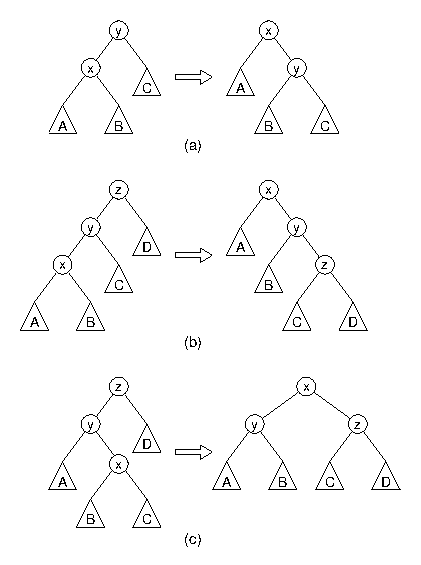
\includegraphics{images/fig1.eps}}
%% \caption{
%% ボトムアップ扁平化操作の1ステップ. % \cite{ST85}
%% $x$ がアクセスした節点.(a) zig: 1回の右回転($y$が根の場合
%% のみ),
%% (b) zig-zig: 枝$yz$と枝$xy$をこの順に右回転,(c) zig-zag: 枝$xy$
%% を左回転し,できた枝$xz$を右回転.}
%% \label{figure:splaying}
%% \end{figure}

%% 扁平化はボトムアップな変形操作であるため,並列操作には適さない.
%% 文献\Cite{ST85}はトップダウン扁平化も提案しているが,これは実装の
%% 容易化が主な目的であり,木の根は操作終了の直前まで確定しない.


%% \subsection{並列操作に関する過去の研究}\label{subsection:related-parallel}

%% 和田\cite{W90}は,並行論理型言語\cite{S89}の論理変数を用いた扁
%% 平化アルゴリズムを提案している.これは,論理変数を利用して,
%% トップダウン扁平化をin-placeで行なうようにしたものと見なすこともできる
%% が,${\it update\/}$のように,対象となる節点が操作終了後の木に存在するこ
%% とがわかっている場合は,木の根のキーを操作の最初に確定させる点が大きな特徴で
%% ある.
%% %
%% % 数百節点の連続挿入操作の並列度は4〜8であるという実験結果が
%% % 報告されている\cite{W90}.
%% %
%% しかしこの技法は,
%% ${\it delete\/}$のように,操作結果の木の根が事前にわから
%% ない場合には適用できない.


%% \subsection{トップダウン扁平化の問題点}

%% トップダウン扁平化による${\it update\/}$は,
%% \ref{subsection:related-parallel}節のように
%% 根のキーを最初に確定させるよ
%% うにしても,並列処理の観点からは問題が残る.たとえば,節点
%% $x(<b)$ ($<$はキーによる順序関係)の${\it update\/}$によって起きる
%% 図\ref{figure:topdown}の
%% zig-zig操作\cite{W90} を考える($L$と$R$は,木$C$をトップダウン扁平
%% 化した結果の左(右)部分木で,${\it update\/}$完了時までに確定).

%% % \begin{adjustvboxheight}
%% \begin{figure}[tb]
%%   \centerline {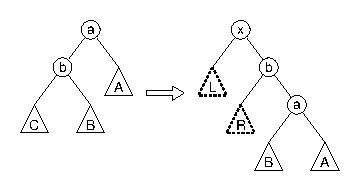
\includegraphics {images/fig2.eps}}
%% \caption{トップダウン扁平化による${\it update\/}$}
%% \label{figure:topdown}
%% \end{figure}
%% % \end{adjustvboxheight}

%% この${\it update\/}$の後,$y(<x)$, $z(>b)$へのアクセスがこの順に続くと
%% する.最初の$x$へのアクセス時に$x$が部分木$C$の左の方にあったためにzig-zig操作
%% が続く場合,$L$の
%% 根が確
%% 定するのは遅くなる.しかし$L$の根が確定するまでは,次の$y$へのアクセ
%% スがzig, zig-zig, zig-zagのどれをまず適用するか決められない.
%% %
%% % 長く待っても,目標の節点の上昇段数が多ければ問題はないのであるが,
%% % それが
%% %
%% そこで3番目の
%% $z$へのアクセスが,2番目の操作によって影響を受けることのない$b$の右部分
%% 木に向かうにもかかわらず,長時間ブロックしてしまう.

%% 削除操作はさらに問題である.一般に,二分木から節点$x$を削除するには,
%% $x$の左部
%% 分木の最大の節点$y$を探してそれを$x$の場所に移すことが基本とな
%% る.しかし,扁平化の有無にかかわらず,$y$が見つかるまでは$x$の場所
%% にくる新たなキーは確定せず,後続の操作をブロックしてしまう.以下のよう
%% な解決法も考えられるが,いずれもうまく動作しない.

%% \begin{enumerate}
%% \item % {\bf 一時的なキー}
%% $y$が見つかるまで,$x$を一時的なキーとして利用すると,
%% $y\le z\le x$であるような節点$z$への操作を誤った方向へ導く.

%% \item % {\bf 双方向リスト}
%% 各節点が直前と直後のキーをもつ節点へのポインタを保持することによって,
%% $x$の直前の要素$y$に${\rm O}(1)$時間でアクセスできるようにする
%% ことが考えられる.これらのポインタは木
%% の扁平化時に変更する必要がないという特徴がある.
%% %
%% しかしこの方法は逐次操作のときしかうまく動作しない.
%% %
%% % あるプロセスが節点
%% % $x$を削除しようとしたとする.そのプロセスは節点$y$に${\rm O}(1)$時間でア
%% % クセスできるものの,単にそれを削除して$x$のかわりに用いることはできない.
%% % (invisible pointer?)
%% %
%% なぜならこの削除操作の前の操作が$x$と$y$を結
%% ぶパスを下降中で,いずれ$y$に到達するかもしれないからである.
%% \end{enumerate}

%% したがって本論文では,高々${\rm O}(1)$個の節を施錠しつつ,厳密にトップダウ
%% ンに木を変形してゆくアルゴリズムを考えることとする.

\section{並列更新アルゴリズム}\label{section:update}

本節では,後続の操作をブロックしない${\it update\/}$操作を与える.基本的な
アイデアは,zig-zigとzig-zagの両方について,目標節点をその深さの
半分までしか浮上させない半扁平化(semi-splaying)を用いることである(文献
\cite{ST85}の半扁平化は,zig-zigのみが扁平化と異なっていた).$x$を更新対
象の節点とすると,アルゴリズムは以下のようになる.
%
% ここでも左右対称な操作の片方のみを述べる.

\begin{itemize}
% \medskip\noindent (a)
\item[(a)]
空の木に対する挿入は図\ref{figure:update}
(a1)の操作,(空でない)木の根に対する更新は
図\ref{figure:update}(a2)の操作を行なう.

% \begin{adjustvboxheight}
\begin{figure*}[t]
  \centerline {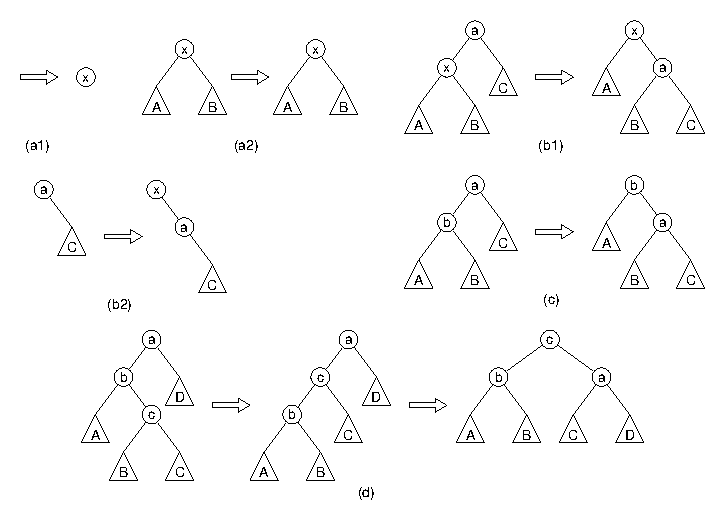
\includegraphics {images/fig3.eps}}
\caption{後続操作をブロックしない更新アルゴリズムの1ステップ}
\label{figure:update}
\end{figure*}
% \end{adjustvboxheight}

% \medskip\noindent (b)
\item[(b)]
zig:
$x$が左部分木の根である場合は図\ref{figure:update}(b1)
の操作,$x$が存在すべき左部分木が空の
場合は図\ref{figure:update}(b2)の操作を行なう.

% \medskip\noindent (c)
\item[(c)]
zig-zig: 図\ref{figure:update}(c)左の木における$x (<b)$の探索では,
枝$ba$の右回転を行なってアクセスしたパスの長さを1短縮する.次は1レベル
(短縮前の長さでは2レベル)下降して,部分木$A$に対して再帰的に探索を行なう.

% \medskip\noindent (d)
\item[(d)]
zig-zag: 図\ref{figure:update}(d)左の木における節点$x$ ($b<x<a$) の
探索では,
枝$cb$の左回転と,できた枝$ca$の右回転を行ない,
アクセスしたパスを1短縮する.
%
% 二つの中側の部分木の適当な方に対して再帰的に探索を行なう.
%
% \noindent
$x=c$ならばこれで探索終了である.$x<c$ならば2レベル(短縮前の長さでは3レ
ベル)下降して$B$の中から$x$を再帰的に
探索する.$x>c$ならば同様に$C$の中から再帰的に探索する.$x\ge c$の場合には
枝$ca$の回転操作を省略することも考えられる.
%
$b$の右部分木が空の場合は,そこに節点$x$を挿入
したあと,上に述べた回転操作を行なう.

\end{itemize}
% \medskip
以上の操作で,アクセスしたパスの長さは最悪でも約$2/3$になる.
%
半分でなくて$2/3$なのは,上記zig-zag操作の性質によるものである.

\section{Coq による形式化}

本節では,3節で述べた \api についてどのように Coq で記述していくかについて説明する.
まず%% 名前,\conf,\conf 中の\free,
仮名関数およびその性質についての Coq での表現を述べる.
次に型付け規則を Coq で使いやすくための規則の具体化を説明し,最後に型システムの健全性の Coq での証明方針を述べる.
また,Coq による定義と証明の全文は GitHub リポジトリ\cite[api]{api}に公開している.
%% また,Coq のバージョンは 8.4pl4 を用いている.
%% 本研究では,アクターの振る舞いに関するこの3つの補題について,Coq を使って形式的な証明を与える.

%% \begin{itemize}
%% \item 振る舞いのインスタンス化について,そのアクターが仮の名前を持つか持たないかによって別個の定義にした
%% \item

%% \section{\conf}

%% \conf は \srcref{coq:conf} のように帰納的に定義した.各コンストラクタの対応関係は 表\ref{coq:conf_table} である.
%% 振る舞いのインスタンス化 $\instantiate{\tilde{u}}{\tilde{v}}{u_1}{z}{P}{\tilde{x}}{\tilde{y}}$ については $len(\tilde{x})$ が1の場合と2の場合で場合分けをしている.

%% \begin{figure}[tbph]
%%   \lstinputlisting[]{./src/config.v}
%%   \caption{\conf}
%%   \label{coq:conf}
%% \end{figure}

%% \begin{table}[tbph]
%%   \caption{\conf の対応関係}
%%   \begin{center}
%%     \begin{tabular}{|ll|}
%%       \hline
%%       $P$                    & {\tt config} \\ \hline
%%       $\nilconf$             & {\tt nil} \\
%%       $\actorconf{x}{y}{P}$  & {\tt create x y P} \\
%%       $\sendconf{x}{y}$      & {\tt send x y} \\
%%       $\restrictconf{x}{P}$  & {\tt restrict x P} \\
%%       $\composeconf{P1}{P2}$ & {\tt compose P1 P2} \\
%%       $\caseconf{x}{y_1 : P_1, ..., y_n : P_n}$ & {\tt caseof x [(y1, P1), ..., (yn, Pn)]} \\
%%       $\instantiate{\tilde{u}}{\tilde{v}}{u_1}{z}{P}{\tilde{x}}{\tilde{y}}$   & {\tt instantiate\_1 u v z p x y}, \\
%%                              & {\tt instantiate\_2 u1 u2 v z p x1 x2 y} \\
%%       \hline
%%     \end{tabular}
%%     \label{coq:conf_table}
%%   \end{center}
%% \end{table}


%% また,名前 $x$ は \conf $P$ 中に現れる\free である,という関係を \srcref{coq:free} のように帰納的に定義した.

%% \begin{figure}[tbph]
%%   \lstinputlisting{./src/free.v}
%%   \caption{\conf と\free の関係}
%%   \label{coq:free}
%% \end{figure}


\subsection{\tmp}

仮につけた名前から正規の名前を得る \tmp の Coq での定義について述べる.

\tmp $ f $ の型は $X \rightarrow X^* $ であり,定義域と値域の集合は $\bot$ と $\ast$ を除くと等しくなっている.
Coq による形式化では簡単にするためにその情報を捨て,任意の {\tt name} 型の値から任意の {\tt option star} 型への関数とした.
定義域の範囲に入っていない入力は {\tt None} を返すことを想定している.
また,ここで {\tt star} 型は {\tt name} 型に $\bot$ と $\ast$ という値を加えたような型である.

この変更により,以下の述語が必要となる.$f : X \rightarrow X^*$ ということを,$in\_range\_in\_domain(f)$ を満たすことで表している.

\begin{dfn}[$in\_domain$]
  名前 $x$ ,\tmp $f$ について,$x \in domain(f)$ を $in\_domain(f,x)$ で表す.ただし $domain(f)$ は $f$ の定義域である.
\end{dfn}

\begin{dfn}[$in\_range$]
  名前 $x$ ,\tmp $f$ について,$x \in range(f)$ を $in\_range(f,x)$ で表す.ただし $range(f)$ は $f$ の値域である.
\end{dfn}

\begin{dfn}[$in\_range\_in\_domain$]
  ある \tmp $f$ が,任意の名前 $x$ について $in\_range(f, x) \Rightarrow in\_domain(f, x)$ を満たすということを \\
  $in\_range\_in\_domain(f)$ で表す.
\end{dfn}

%% \begin{figure}[tbph]
%%   \lstinputlisting{./src/range_domain.v}
%%   \caption{述語 $in\_domain, in\_range, in\_range\_in\_domain$}
%%   \label{coq:range_domain}
%% \end{figure}

また,2つの \tmp の定義域が重なっていないことを表す述語 $fun\_exclusive$ を定義する.

\begin{dfn}[$fun\_exclusive$]
  2つの \tmp $f : X \rightarrow X^*, g : Y \rightarrow Y^*$ について,$X \cap Y = \emptyset$ であるという述語を $fun\_exclusive$ と定義する.
%% 述語をある名前 $x$ が $f$ の定義域の要素であるならば $x$ は $g$ の定義域の要素ではない,かつ,$x$ が $g$ の定義域の要素であるならば $x$ は $f$ の定義域のではない,
\end{dfn}

%% これは述語 $in\_domain$ を使って \srcref{coq:fun_exclusive} のように定義できる.

%% \begin{figure}[tbph]
%%   \lstinputlisting{./src/fun_exclusive.v}
%%   \caption{$fun\_exclusive$}
%%   \label{coq:fun_exclusive}
%% \end{figure}

  %% $ \bot, \ast \notin {\cal N}, X \subset {\cal N}, X^* = X \cup \{\bot,\ast\} $
  %% \begin{table}[htb]
  %%   \begin{tabular}{ll}
  %%     $ f(x) $ & if $ x $ is a regular actor name \\
  %%     $ f(x) = \ast $ & if $ x $ is the temporary name \\
  %%     \ & of an actor with a private name \\
  %%     $ f(x) = y \notin \{\bot,\ast\} $ & means that actor $ y $ has assumed \\
  %%     \ & the temporary name $ x $
  %%   \end{tabular}
  %% \end{table}
  %% and $ f^* : X^* \rightarrow X^* $ as $ f^*(x) = f(x) \  for \ x \in X $ and $ f^*(\bot) = f^*(\ast) = \bot $

\subsubsection{\tmp の構築}

\tmp は $ch$ 関数,\tmp の合成,\tmp の定義域の制限,のいずれかで作ることができる.
ここで,$ch$ 関数が使われている型付け規則は \textsc{Act} のみであるが,この中で使われている $ch$ 関数は入力の要素数が0個,1個,2個のものしかない.
よって,$ch$ 関数はこの3パターンに限定でき,それぞれ $ch_0, ch_1, ch_2$ と書くこととする.
また,\tmp の定義域の制限を行う二項演算子 $(|)$ が現れるのは \textsc{Res} のみで,かつそれはもとの仮名関数の定義域からあるひとつの要素を取り去るものとしてしか使われていない.
後の証明を簡単にするために,この演算子を,制限後の集合ではなく定義域から取り去る要素を右手にとるものとして定義する.
ただし,この演算子はもとの演算子 $(|)$ とは定義が異なるため,混乱を避けるために別の記号 $(\setminus)$ を用いることにする.

\begin{dfn}[\tmp の定義域の制限]
  $f : \rho \rightarrow \rho^*, x \in \rho$ である $f, x$ に対して定義域の制限を表す二項演算子 $f \setminus x : \rho - \{x\} \rightarrow (\rho - \{x\})^*$ を以下のように定義する. \\
\begin{adjustvboxheight}
  \[ (f \setminus x)(y) = \begin{cases}
    \ast & f(y) = x \mbox{のとき} \\
    f(y) & \mbox{その他}
  \end{cases} \]
  \vspace{1pt}
\end{adjustvboxheight}
\end{dfn}


また,$ch_0, ch_1, ch_2, \oplus, \setminus$ について仮名関数の性質を満たすことを証明した.
その際,$ch_2$ は引数である2つの名前が異なることを,$\oplus$ は $in\_domain\_in\_range, fun\_exclusive$ が成り立つという前提を加えている.

%% 以上の5つを \srcref{tmp_fun} と定義した.


%% %% 型付け規則 \textsc{Act} を分割した \textsc{Act-empty}, \textsc{Act-x}, \textsc{Act-z}, \textsc{Act-xz} のみであるが,これらの規則内の

%% \begin{figure}[tbph]
%%   \lstinputlisting{./src/tmp_fun.v}
%%   \caption{\tmp の構築}
%%   \label{tmp_fun}
%% \end{figure}

%% \subsection{\tmp の性質}

%% \tmp を構築するものは,5種しかなかったが,これら全てにおいて\tmp の性質を満たす.\tmp の性質は Coq では \srcref{coq:tmp_prop} と定義した.

%% \begin{figure}[tbph]
%%   \lstinputlisting{./src/tmp_prop.v}
%%   \caption{\tmp の性質}
%%   \label{coq:tmp_prop}
%% \end{figure}

%% それぞれの要素を用いて構築された\tmp について,それが\tmp の性質を満たすという補題を証明する必要がある.

%% \begin{lem}[\tmp の性質($ch_0$)]
%%   \label{lemma:ch_0_prop}
%%   $ch_0$ は \tmp の性質を満たす.
%% \end{lem}

%% \begin{lem}[\tmp の性質($ch_1$)]
%%   \label{lemma:ch_1_prop}
%%   $ch_1$ は \tmp の性質を満たす.
%% \end{lem}

%% \begin{lem}[\tmp の性質($ch_2$)]
%%   \label{lemma:ch_2_prop}
%%   $ch_2$ は,2つの入力 $x, y$ について $x \neq y$ であるならば,\tmp の性質を満たす.
%% \end{lem}

%% \begin{lem}[\tmp の性質($fun\_plus$)]
%%   \label{lemma:fun_plus_prop}
%%   \tmp $f, g$ が \tmp の性質,$range\_domain$,$fun\_exclusive$ を満たすならば,$fun\_plus(f, g)$ は \tmp の性質を満たす.
%% \end{lem}

%% \begin{lem}[\tmp の性質($fun\_remove$)]
%%   \label{lemma:fun_remove_prop}
%%   \tmp $f$ が \tmp の性質満たすならば,任意の名前 $x$ について $fun\_remove(f, x)$ は \tmp の性質を満たす.
%% \end{lem}

%% これらの補題は,Coq では\srcref{coq:fun_prop} のように定義した.

%% \begin{figure}[htbp]
%%   \lstinputlisting{./src/fun_prop.v}
%%   \caption{\tmp の性質の補題}
%%   \label{coq:fun_prop}
%% \end{figure}


%% 以下の補題は \tmp の Coq での定義に,定義域と値域の情報が入っていないことによる補題(元の定義では自明)


%% また,二つの\tmp $f_1, f_2$ が互換性を持つという述語,及び\tmp $f_1, f_2, ..., f_n$ が相互に互換性を持つという述語を,\srcref{coq:compatible} と定義した.

%% \begin{figure}[tbph]
%%   \lstinputlisting{./src/compatible.v}
%%   \caption{互換性}
%%   \label{coq:compatible}
%% \end{figure}


\subsection{型付け規則}

%% 本節では,\api の型付け規則を Coq で定義する.

\api の型付け規則には,Coq 上で定義しにくい,またはそのままでは証明を進めにくいものがある.実際に Coq で型付け規則を定義する前に,型付け規則を再定義する.

\subsubsection{\textsc{Act} 規則の分割}

型付け規則 \textsc{Act} はアクターが作られる際に考えられるパターンを複数まとめたものであり,このままの定義を用いると証明が煩雑になってしまう.
これは,\textsc{Act} に関する証明を行う際に,$ch$ 関数の定義にともなって \textsc{Act} に現れる $\rho$ の要素数で場合分けをすることになるが,その都度考えられない場合が現れ,その場合は矛盾を証明する,ということをしなければならないためである.
また,Coq では任意の要素数を持つ集合を扱うような証明は煩雑になってしまいやすい.
そこで,事前に $\rho$ の要素数によって場合分けを行い,\textsc{Act} を分割しておくことを考える.
$\rho$ の場合分けを行うと,以下のように4つに分けられることがわかる.

\begin{enumerate}
  \item 要素数が0のとき \\
    $\rho - \{x\} = \hat{z}$ から,$\hat{z} = \emptyset, f = ch_0$ である.
  \item 要素数が1のとき
    \begin{enumerate}
      \item $x \in \rho$ のとき \\
        $\rho - \{x\} = \hat{z}$ で $len(\rho) = 1$ なので,$\hat{z} = \emptyset, f = ch_1(x)$ である.
      \item $x \notin \rho$ のとき \\
        $\rho - \{x\} = \hat{z}$ であるから,$len(\hat{z}) = 1$ である.$\hat{z} = \{z\}$ とすると,$f = ch_1(z)$ である.
    \end{enumerate}
  \item 要素数が2のとき \\
    $\rho - \{x\} = \hat{z}$ であり,$\hat{z}$ は要素数が $0$ または $1$ なので,$x \in \rho$ である.$\hat{z} = \{z\}$ とすると,$f = ch_2(x,z)$ である.
  \item 要素数が3以上のとき \\
    $3 \leq len(\rho)$ のとき,$\hat{z} (= \rho - \{x\})$ は要素数が2以上である.これは $\hat{z}$ の定義と矛盾する.よって要素数が3以上であることはない.
\end{enumerate}


この場合分けをもとに,\textsc{Act} を4つに分割すると,\srcref{coq:act} のような定義にできる.

\begin{figure}[t]
  \infrule[Act-empty]{
    \typing{\emptyset}{ch_0}{P}
  }{
    \typing{\{x\}}{ch_1(x)}{x(y).P}
  }
  \vspace{14pt}
  \infrule[Act-x]{
    \typing{\{x\}}{ch_1(x)}{P}
    \andalso x \neq y
  }{
    \typing{\{x\}}{ch_1(x)}{x(y).P}
  }
  \vspace{14pt}
  \infrule[Act-z]{
    \typing{\{z\}}{ch_1(z)}{P}
    \andalso x \neq z
    \andalso y \neq z
  }{
    \typing{\{x, z\}}{ch_2(x, z)}{x(y).P}
  }
  \vspace{14pt}
  \infrule[Act-xz]{
    \typing{\{x, z\}}{ch_2(x, z)}{P}
    \andalso x \neq z
    \andalso x \neq y
    \andalso y \neq z
  }{
    \typing{\{x, z\}}{ch_2(x, z)}{x(y).P}
  }

  \caption{型付け規則\textsc{Act} の分割}
  \label{coq:act}
\end{figure}


\subsubsection{\textsc{Case} 規則の分割}

型付け規則 \textsc{Case} は,前提の数がパターンの数に依存して変動するので,Coq で定義しにくい.よって \srcref{api:case_split} のように \textsc{Case} をパターンが $0$ 個の場合と $i + 1$ に分割し,帰納的に定義する.これで,\textsc{Case} 規則の前提の数はパターンの数によらず一定となる.


\begin{figure}[t]
  \infrule[Case-nil]{
  }{
    \typing{\emptyset}{\{\}}{\caseconf{x}{}}
  }
  \vspace{14pt}
  \infrule[Case-cons]{
    \typing{\rho}{f}{\caseconf{x}{y_1 : P_1, ... , y_i : P_i}}
    \\
    \andalso \typing{\rho'}{f'}{P}
    \andalso compatible(f, f')
  }{
    \typing{\rho \cup \rho'}{f \oplus f'}{\caseconf{x}{y : P, y_1 : P_1, ... , y_i : P_i}}
  }

  \caption{型付け規則\textsc{Case} の分割}
  \label{api:case_split}
\end{figure}


また,この定義によって作られる型付け
\begin{center}
  $\typing{(...((\rho_1 \cup \rho_2) \cup \rho_3)... \cup \rho_n) \cup \rho}{(...((f_1 \oplus f_2) \oplus f_3)... \oplus f_n) \oplus f}{\caseconf{x}{y : P, y_1 : P_1, ..., y_n : P_n}}$
\end{center}
において,元の定義では $f, f_1, f_2, ..., f_n$ が相互に互換性を持つことを条件としているが,
$f, f_1, ..., f_n$ が相互に互換性を持つことは自明ではない.よって以下の補題が必要となる.

\begin{lem}
  仮名関数 $f, f_1, f_2$ について,$f$ と $f_1 \oplus f_2$ が互換性を持ち,$f_1$ と $f_2$ もまた互換性を持つとき,$f, f_1, f_2$ は相互に互換性を持つ.
  \label{lem:compatible}
\end{lem}

この補題の Coq による証明は \texttt{Fun} モジュールの \texttt{fun\_plus\_compatible} という名前にあるが,以下にその概略を示す.

まず $f$ と $f_1$ が $\oplus$ について可換であること, $f$ と $f_2$ が $\oplus$ について可換であることを,$f$ と $f_1 \oplus f_2$ が互換性を持ち $f_1$ と $f_2$ もまた互換性を持つという仮定から示す.このことから,$f$,$f_1$,$f_2$ が相互に可換になることがわかる.
次に,$f$,$f_1$,$f_2$ の任意の組み合わせの合成が\tmp の性質を満たすことを証明する.まずは $f$ と $f_1$ の合成が仮名関数の性質を満たすことを証明する.
$f$ と $f_1 \oplus f_2$ が互換性を持つという仮定から,$f \oplus (f_1 \oplus f_2)$ が仮名関数の性質を満たす.また仮名関数の合成は結合律が成り立つので $(f \oplus f_1) \oplus f_2$ も仮名関数の性質を満たす.
合成が仮名関数の性質を満たしているならば合成の左手は仮名関数の性質を満たす,という性質 (\texttt{fun\_prop\_plus\_fst} という名前で証明済み) を,先に証明した $(f \oplus f_1) \oplus f_2$ も仮名関数の性質を満たすということに使うと,$f \oplus f_1$ が仮名関数の性質を満たすということを導ける.
$f$ と $f_2$ についても同様である.また,$f_1$ と $f_2$ については仮定から明らかである.
以上から,$f$,$f_1$,$f_2$ の任意の組み合わせの合成が\tmp の性質を満たすことがわかったので,$f$,$f_1$,$f_2$ が相互に可換になることと合わせると,$f$,$f_1$,$f_2$ は相互に互換性を持つことがわかる.

この補題によって,$f, f_1, ... , f_n$ が相互に互換性を持つことが帰納的に保証される.%% この補題は Coq では \srcref{coq:fun_plus_compatible} と定義できる.

%% \begin{figure}[tbph]
%%   \lstinputlisting{./src/fun_plus_compatible.v}
%%   \caption{補題 \ref{lem:compatible} の Coq での定義}
%%   \label{coq:fun_plus_compatible}
%% \end{figure}


\subsubsection{\textsc{Res} 規則}

\tmp の定義域の制限を行う二項演算子の定義を変更したことに合わせて,型付け規則 \textsc{Res} は \srcref{api:res_rule} のようになる.

\begin{figure}[t]
  \infrule[Res]{
    \typing{\rho}{f}{P}
  }{
    \typing{\rho - \{x\}}{f \setminus x}{\restrictconf{x}{P}}
  }
  \caption{型付け規則 \textsc{Res}}
  \label{api:res_rule}
\end{figure}

\subsubsection{\textsc{Inst} 規則の分割}

Coq による定義では振る舞いの雛形からアクターを作る\conf $\behaviorconf{\tilde{x}}{\tilde{y}} (B \defeq \behaviortemplate{\tilde{u}}{\tilde{v}}{u_1}{z}{P})$ を,$\tilde{u}$ の要素数が1である場合と2である場合で二つに分割している.
よって型付け規則も二つに分割する必要があり,\srcref{api:inst_rule} のようになる.
ただし,ここでは $B$ を使う代わりに $B$ の展開後の項を用いている.

\begin{figure}[t]
  \infrule[Inst-1]{
    \typing{\{u\}}{ch_1(u)}{\actorconf{u}{z}{P}}
  }{
    \typing{\{x\}}{ch_1(x)}{\instantiate{\tuple{u}}{\tilde{v}}{u}{z}{P}{\tuple{x}}{\tilde{y}}}
  }
  \vspace{14pt}
  \infrule[Inst-2]{
    \typing{\{u_1,u_2\}}{ch_2(u_1,u_2)}{\actorconf{u_1}{z}{P}}
    \andalso x_1 \neq x_2
  }{
    \typing{\{x_1, x_2\}}{ch_2(x_1, x_2)}{\\ \ \ \ \ \ \ \ \ \instantiate{\tuple{u_1,u_2}}{\tilde{y}}{u_1}{z}{P}{\tuple{x_1,x_2}}{\tilde{y}}}
  }
  \caption{型付け規則 \textsc{Inst} の分割}
  \label{api:inst_rule}
\end{figure}


%% \subsection{型付け規則の Coq での定義}

%% 分割後を含めた型付け規則全体の Coq 上での定義を \srcref{typing} に示す.型付け規則を素直に表現することで定義することができた.

%% \begin{figure}[tbph]
%%   \ContinuedFloat
%%   \lstinputlisting[basicstyle=\small]{./src/typing.v}
%%   \caption{型付け規則}
%%   \label{typing}
%% \end{figure}

\subsection{健全性の証明}


最後に健全性の証明を行うが,以下の3つの補題を証明しておくと,健全性の証明を行いやすいので証明しておく.対応する Coq による証明は,\texttt{Typing.v} ファイルの \texttt{typing\_in\_range\_in\_domain},\texttt{typing\_in\_domain\_1} および \texttt{typing\_in\_domain\_2},\texttt{Soundness.v} ファイルの \texttt{typing\_fun\_exclusive} にある.
%% \begin{figure}[tbph]
%%   \lstinputlisting{./src/fun_ext.v}
%%   \caption{関数の外延的同値}
%%   \label{coq:fun_ext}
%% \end{figure}


\begin{lem}[定義域と値域の一致]
  \label{lemma:typing_range_domain}
  $\typing{\rho}{f}{P}$ ならば,$in\_range\_in\_domain(f)$ が成り立つ.
\end{lem}

\begin{lem}[\tmp の定義域と\recep の一致]
  \label{lemma:typing_recep_domain}
  $\typing{\rho}{f}{P}$ ならば,任意の名前 $ x $ について $in\_domain(f, x) $ であるとき,かつそのときに限り,$ x \in \rho $ が成り立つ.
\end{lem}

\begin{lem}[$fun\_exclusive$ における集合の一致]
  \label{lemma:typing_fun_exclusive}
  $\typing{\rho_1}{f_1}{P_1}$ かつ $\typing{\rho_2}{f_2}{P_2}$ であり $ \rho_1 \cap \rho_2 \neq \emptyset $ ならば,$fun\_exclusive(f_1, f_2)$ を満たす.
\end{lem}

健全性は,以上の公理と補題を利用して,型付け規則の構造に関する帰納法で証明できる.対応する Coq の証明は \texttt{Soundness.v} ファイルの \texttt{Soundness} にある.

%% これらの補題は,Coq では \srcref{coq:lemma} のように定義した.


%% \begin{figure}[tbph]
%%   \lstinputlisting{./src/lemma.v}
%%   \caption{健全性の証明に必要となる補題}
%%   \label{coq:lemma}
%% \end{figure}

%% \subsection{Coq での定義と証明}

%% \api の健全性の定理は,\srcref{soundness} のように定義した.

%% \begin{figure}[tbph]
%%   \lstinputlisting{./src/soundness.v}
%%   \caption{健全性}
%%   \label{soundness}
%% \end{figure}

%% 証明の全文は付録Aに示した.ここでは\api の健全性の3つの要素である \recep の健全性,仮名の取り方についての健全性,型付けの一意性のそれぞれについて証明の方針について示す.

%% \subsubsection{\recep の健全性}

%% \recep の健全性は,次の方針で証明できる.

%% \begin{proof}
%%   型付けの構造に関する帰納法で証明する.

%%   \begin{enumerate}
%%     \item[(\textsc{Nil})]
%%       \recep は空集合なので明らか.
%%     \item[(\textsc{Msg})]
%%       \textsc{Nil} と同様に明らか.
%%     \item[(\textsc{Act-empty})]
%%       $\typing{\{x\}}{ch_1(x)}{\actorconf{x}{y}{P}}$ で,$x$ は $\actorconf{x}{y}{P}$ の\free であるので,命題を満たす.
%%     \item[(\textsc{Act-x})]
%%       \textsc{Act-empty} と同様に命題を満たす.
%%     \item[(\textsc{Act-z})]
%%       帰納法の仮定から,$z$ は $P$ の\free であり,$y \neq z$ という条件から,$z$ は $\actorconf{x}{y}{P}$ 中の\free である.
%%       また,$x$ も $\actorconf{x}{y}{P}$ 中の\free であるので,命題を満たす.
%%     \item[(\textsc{Act-xz})]
%%       \textsc{Act-z} と同様に命題を満たす.
%%     \item[(\textsc{Case-nil})]
%%       \textsc{Nil} と同様に明らか.
%%     \item[(\textsc{Case-cons})]
%%       帰納法の仮定から $\rho$ のすべての要素は $\caseconf{x}{y_1 : P_1, ..., y_i : P_i}$ 中の\free であり,$\rho'$ のすべての要素は $P$ 中の\free である.
%%       $\rho$ のすべての要素および $\rho'$ のすべての要素は,$\caseconf{x}{y : P, y_1 : P_1, ..., y_i : P_i}$ の\free であるので,$\rho \cup \rho'$ についてもこれを満たす.
%%     \item[(\textsc{Comp})]
%%       帰納法の仮定から,$\rho_1$ のすべての要素は $P_1$ の\free であり,$\rho_2$ のすべての要素は $P_2$ の\free である.
%%       よって $\rho_1 \cup \rho_2$ のすべての要素は $\composeconf{P_1}{P_2}$ の\free である.
%%     \item[(\textsc{Res})]
%%       帰納法の仮定から,$\rho$ のすべての要素は $P$ 中の\free である.
%%       $\restrictconf{x}{P}$ によって $x$ は\free ではなくなるが,$x$ は $\rho - \{x\}$ の要素ではないため,命題を満たす.
%%     \item[(\textsc{Inst-1})]
%%       $\typing{\{x\}}{ch(x)}{\instantiate{\tuple{u}}{\tilde{v}}{u}{z}{P}{\tuple{x}}{\tilde{y}}}$ で,$x$ は
%%       $\instantiate{\tuple{u}}{\tilde{v}}{u}{z}{P}{\tuple{x}}{\tilde{y}}$ の\free であるので,命題を満たす.
%%     \item[(\textsc{Inst-2})]
%%       $\typing{\{x_1,x_2\}}{ch_2(x_1,x_2)}{\instantiate{\tuple{u_1,u_2}}{\tilde{v}}{u_1}{z}{P}{\tuple{x_1,x_2}}{\tilde{y}}}$ で,$x_1,x_2$ は \\
%%       $\instantiate{\tuple{u_1,u_2}}{\tilde{v}}{u_1}{z}{P}{\tuple{x_1,x_2}}{\tilde{y}}$ の\free であるので,命題を満たす.
%%   \end{enumerate}
%% \end{proof}

%% \subsubsection{仮名の取り方の健全性}

%% 仮名の取り方の健全性は以下の方針で証明できる.

%% \begin{proof}
%%   型付けの構造に関する帰納法で証明する.

%%   \begin{enumerate}
%%     \item[(\textsc{Nil})]
%%       \lemmaref{lemma:ch_0_prop} より明らか.
%%     \item[(\textsc{Msg})]
%%       \textsc{Nil} と同様に明らか.
%%     \item[(\textsc{Act-empty})]
%%       \lemmaref{lemma:ch_1_prop} より明らか.
%%     \item[(\textsc{Act-x})]
%%       \lemmaref{lemma:ch_1_prop} より明らか.
%%     \item[(\textsc{Act-z})]
%%       \lemmaref{lemma:ch_2_prop} より明らか.
%%     \item[(\textsc{Act-xz})]
%%       \lemmaref{lemma:ch_2_prop} より明らか.
%%     \item[(\textsc{Case-nil})]
%%       \textsc{Nil} と同様に明らか.
%%     \item[(\textsc{Case-cons})]
%%       互換性の定義より明らか.
%%     \item[(\textsc{Comp})]
%%       \lemmaref{lemma:fun_plus_prop} ,\lemmaref{lemma:typing_range_domain} ,\lemmaref{lemma:typing_fun_exclusive} を使って証明できる.
%%     \item[(\textsc{Res})]
%%       \lemmaref{lemma:fun_remove_prop} より明らか.
%%     \item[(\textsc{Inst-1})]
%%       \lemmaref{lemma:ch_1_prop} より明らか.
%%     \item[(\textsc{Inst-2})]
%%       \lemmaref{lemma:ch_2_prop} より明らか.
%%   \end{enumerate}
%% \end{proof}

%% \subsubsection{型付けの一意性}

%% 型付けの一意性は以下の方針で証明できる.

%% \begin{proof}
%%   型付けの構造に関する帰納法で証明する.

%%   \begin{enumerate}
%%     \item[(\textsc{Nil})]
%%       $\nilconf$ の型付け規則は \textsc{Nil} 規則のみで,さらに\recep は空集合,\tmp は空関数なので,命題を満たす.
%%     \item[(\textsc{Msg})]
%%       $\sendconf{x}{y}$ ($x, y$ は任意) の型付け規則は \textsc{Msg} のみで,さらに\recep は空集合,\tmp は空関数なので,命題を満たす.
%%     \item[(\textsc{Act-empty})]
%%       この型付け規則の前提は $\typing{\emptyset}{ch_0}{P}$ であり,帰納法の仮定から,この $P$ の型付けは唯一である.
%%       $\typing{\{x\}}{ch_1(x)}{\actorconf{x}{y}{P}}$ となる型付け規則は \textsc{Act-empty}, \textsc{Act-x} の2種類あるが,$\typing{\emptyset}{\{\}}{P}$ から構築できるのは \textsc{Act-empty} のみであり,かつ\recep と\tmp は $x$ で構築されている.よって命題を満たす.
%%     \item[(\textsc{Act-x})]
%%       この型付け規則の前提は $\typing{\{x\}}{ch_1{x}}{P}$ であり,帰納法の仮定から,この $P$ の型付けは唯一である.
%%       $\typing{\{x\}}{ch_1(x)}{\actorconf{x}{y}{P}}$ となる型付け規則は \textsc{Act-empty}, \textsc{Act-x} の2種類あるが,$\typing{\{x\}}{ch_1(x)}{P}$ から構築できるのは \textsc{Act-x} のみであり,かつ\recep と\tmp は $x$ で構築されている.よって命題を満たす.
%%     \item[(\textsc{Act-z})]
%%       この型付け規則の前提は $\typing{\{z\}}{ch_1(z)}{P}$ であり,帰納法の仮定から,この $P$ の型付けは唯一である.
%%       $\typing{\{x,z\}}{ch_2(x,z)}{\actorconf{x}{y}{P}}$ (ただし $x \neq z$) となる型付け規則は \textsc{Act-z}, \textsc{Act-xz} の2種類あるが,$\typing{\{z\}}{ch_1(z)}{P}$ から構築できるのは \textsc{Act-z} のみであり,かつ\recep と\tmp は $x,z$ で構築されている.よって命題を満たす.
%%     \item[(\textsc{Act-xz})]
%%       この型付け規則の前提は $\typing{\{x,z\}}{ch_2(x,z)}{P}$ (ただし $x \neq z$) であり,帰納法の仮定から,この $P$ の型付けは唯一である.
%%       $\typing{\{x,z\}}{ch_2(x,z)}{\actorconf{x}{y}{P}}$ となる型付け規則は \textsc{Act-z}, \textsc{Act-xz} の2種類あるが,$\typing{\{x,z\}}{ch_2(x,z)}{P}$ から構築できるのは \textsc{Act-xz} のみであり,かつ\recep と\tmp は $x,z$ で構築されている.よって命題を満たす.
%%     \item[(\textsc{Case-nil})]
%%       $\caseconf{x}{}$ ($x$ は任意) の型付け規則は \textsc{Case-nil} のみで,さらに\recep は空集合,\tmp は空関数なので,命題を満たす.
%%     \item[(\textsc{Case-cons})]
%%       この型付け規則の前提は $\typing{\rho}{f}{\caseconf{x}{y_1 : P_1, ... , y_i : P_i}}$ および $\typing{\rho'}{f'}{P}$ であり,帰納法の仮定からこれらの型付けは一意である.
%%       $\typing{\rho \cup \rho'}{f \oplus f'}{\caseconf{x}{y : P, y_1 : P_1, ... , y_i : P_i}}$ となる型付け規則は \textsc{Case-cons} のみであり,かつ\recep は $\rho, \rho'$ ,\tmp は $f,f'$ で構築されている.よって命題を満たす.
%%     \item[(\textsc{Comp})]
%%       この型付け規則の前提は $\typing{\rho_1}{f_1}{P_1}$ および $\typing{\rho_2}{f_2}{P_2}$ であり,帰納法の仮定からこれらの型付けは一意である.
%%       $\typing{\rho_1 \cup \rho_2}{f_1 \oplus f_2}{P_1 \setminus P_2}$ となる型付け規則は \textsc{Comp} のみであり,かつ\recep は $\rho_1, \rho_2$ ,\tmp は $f_1,f_2$ で構築されている.よって命題を満たす.
%%     \item[(\textsc{Res})]
%%       この型付け規則の前提は $\typing{\rho}{f}{P}$ ,帰納法の仮定からこの型付けは一意である.
%%       $\typing{\rho - \{x\}}{f \setminus x}{(\nu x)P}$ となる型付け規則は \textsc{Res} のみであり,かつ\recep と\tmp は共に $\rho, x$ で構築されている.よって命題を満たす.
%%     \item[(\textsc{Inst-1})]
%%       $\instantiate{\tuple{u}}{\tilde{v}}{u}{z}{P}{\tuple{x}}{\tilde{y}}$ の型付け規則は \textsc{Inst-1} のみで,かつ\recep と\tmp は $x$ のみで構築されているので,命題を満たす.
%%     \item[(\textsc{Inst-2})]
%%       $\instantiate{\tuple{u_1,u_2}}{\tilde{v}}{u_1}{z}{P}{\tuple{x_1,x_2}}{\tilde{y}}$ (ただし $x_1 \neq x_2$) の型付け規則は \textsc{Inst-2} のみで,かつ\recep と\tmp は $x_1,x_2$ のみで構築されているので,命題を満たす.
%%   \end{enumerate}
%% \end{proof}

%% 以上から,健全性の定理での3つの命題を満たすので,\api の型システムは健全性を満たすことを証明できる.









%% \section{並列削除アルゴリズム}\label{section:delete}

%% 並列削除のための基本的な着想は,扁平化操作を,削除すべき節点を下降さ
%% せるために利用することである.これまでは,扁平化操作はもっぱら,再度アク
%% セスしそう
%% な節点を浮上させるために用いられてきた.ここで重要なことは,削除対象の
%% 節点以外は高々${\rm O}(1)$レベルしか下降させないようにすることである.
%% 以下では,$z$を削除対象の節点とする.

%% まず,根節点が削除対象節点$z$である場合を考える.この場合,zippingと呼ぶ
%% 操作によって
%% それを``容易に''削除できる場所まで下降させる.節点が``容易に''削除でき
%% るとは,その左部分木,右部分木,左部分木の右部分木,右部分木の左部分木の
%% いずれかが空であることである.根節点の下降によって,その左部分木と
%% 右部分木の縫い合せが起きる.
%% %
%% % これが言葉の由来である.

%% \begin{enumerate}
%% % \medskip\noindent (a)
%% \item[(a)]
%% ``容易に''削除できる場合:図\ref{figure:delete}(a1)または(a2)
%% のように変形する.


%% % \begin{adjustvboxheight}
%% \begin{figure*}[t]
%%   \centerline {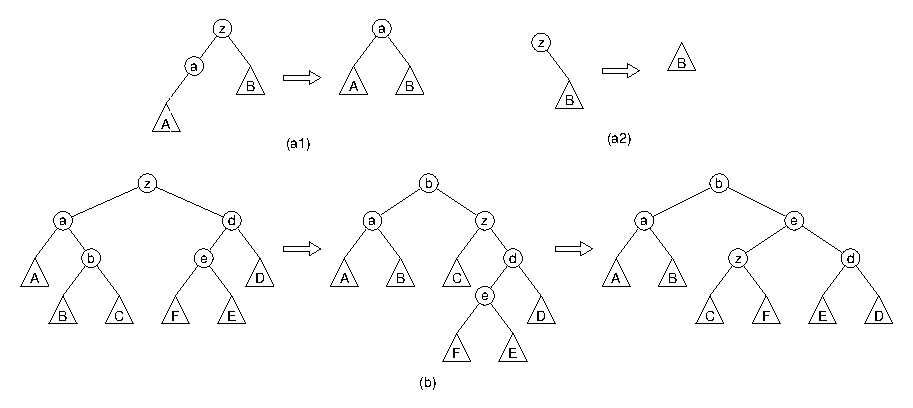
\includegraphics {images/fig4.eps}}
%% \caption{後続操作をブロックしない削除アルゴリズムの1ステップ}
%% \label{figure:delete}
%% \end{figure*}
%% % \end{adjustvboxheight}

%% % \medskip\noindent (b)
%% \item[(b)]
%% ``容易に''削除できない場合:図\ref{figure:delete}(b)のように
%% zig-zagを施し,そ
%% の結果できる$b$の右部分木に,(一つめとは左右対称な) zig-zagを施す.

%% \noindent
%% 4回の回転で$z$は2レベル下降する.$z$の新たな部分木$C$と$F$
%% は,同じレベルにとどまる.それ以外の節点も高々1レベルしか下降
%% しない.$z$を根とする新たな部分木に対して再帰的に削除操作を行なうが,$z$の子孫
%% でない節点がそれによってさらに下降することはない.
%% \end{enumerate}

%% % \medskip
%% 図\ref{figure:zipping}に,根節点$z$の削除による木の形状の変化を示す.
%% \begin{figure*}[t]
%%   \centerline {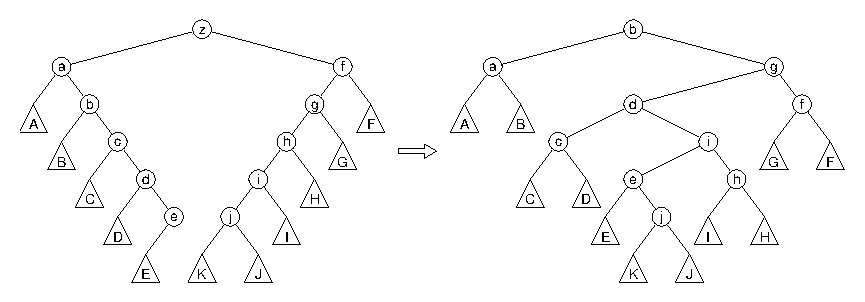
\includegraphics {images/fig5.eps}}
%% \caption{Zippingによる節点$z$の削除}
%% \label{figure:zipping}
%% \end{figure*}

%% 削除対象節点$z$が根であるとは限らない場合は,まず第\ref{section:update}節の
%% 方法で$z$を探索する.これは根から$z$に至るパスを短縮する効果をもつ.つぎ
%% に,$z$をzippingによって下降させて削除する.

%% Zipping操作はパスの短縮を行なわないが,アクセスした節点は浮上させ
%% るという原則にしたがうならば,zippingに先だって,左部分木の最大要素に至
%% るパスと右部分木の最小要素に至るパスをそれぞれトップダウンの半扁平化
%% (zig-zig (図\ref{figure:update}(c)) の繰返し)によっ
%% て短縮すればよい.この短縮化はzippingと並行して行なうことができる.

%% Zippingは更新操作と異なり,各節点のキー値を読むことなく木を下降する.
%% またzippingは,木$T_1$と木$T_2$ ($T_1$のど
%% のキーも,$T_2$のどのキーよりも小さいものとする)とのトップダウン併合操作
%% にも応用できる.すなわち,新たな節点(キーは任意)を調達し,その左部分木
%% を$T_1$,右部分木を$T_2$として一つの木を構成した
%% のち,調達した根節点を消去すればよい.

%% \section{まとめ}

%% %% 本章では,本研究の今後の課題と結論について述べる.

%% \section{課題}

%% \subsection{操作的意味論}

%% 本研究では \api の型システムを検証したが,その操作的意味論には触れていない.\api の操作的意味論は,$\pi$ 計算と同様にラベル付き遷移 (labeled transition system) を用いている.\api は,型がついているものは遷移先でも型がついているという型保存 (preservation) が成り立つ.このような\api の操作的意味論の Coq での定式化,および型保存性の証明が課題として残っている.


%% \subsection{抽出}

%% Coq は,抽出 (extraction) という機能を持っている.これは,Coq で定義した関数や証明を,対象のプログラミング言語のコードに変換する,というものである.対象のプログラミング言語は OCaml,Haskell,Scheme などがある.Coq は副作用を起こすようなコードは書くことができないので,副作用が必要な場合は他のプログラミング言語のコードに変換し,その言語の機構を用いる必要がある.

%% 本研究で定義した関数および証明を抽出し,別のプログラミング言語のコードに変換することによって,正しさが証明された \api を実装することができると考えられる.

\section{結論}

\api における型システムの定義を Coq で証明を行いやすいように再定義し,\api の型付けの健全性を形式的に証明した.これによって \api の型システムが確かにアクターとしての振る舞いを強制することを示した.

%% \section{計算量に関する結果と考察}

%% 効率の二つの尺度のうち,スループットにつ
%% いては容易に議論ができる.すなわち,二つの操作は,レベル$l$ (根をレ
%% ベル$0$として)の節点を${\rm O}(l)$回 --- ${\it update\/}$は高々$(l+2)$回,
%% zippingは高々$(2l+2)$回 ---
%% の回転操作ののちに確定させる.
%% さらにどちらの操作も,連続する高々$3$
%% レベルの節点を同時に施錠するだけでよい.これらのことから,木の大きさや深
%% さによらないスループットで,操作系列をパイプライン的に並列処理するこ
%% とができる.

%% レスポンスは,${\it update\/}$については,通常のスプレー
%% 木と同等の償却計算量をもつことが証明できる.具体的には,
%% 節点$x$の{\bf 大きさ}$s(x)$を$x$を根とする部分木の節点数と定義し,
%% {\bf ランク}$r(x)$を$\log_2(s(x))$とする.
%% そして
%% %
%% 木の{\bf ポテンシャル}を,すべての節点のランクの和と定義する.
%% すると,${\it update\/}$の償却時間,つまり回転操作の回数で測った所
%% 要時間に操作前後のポテンシャルの変化を加えたものは,$n$を木の節点数とし
%% て,${\rm O}(\log n)$であることを示すことができる.
%% このことから,十分長い操作系列の平均レスポンスは,最悪でも対数的であるこ
%% とがわかる.
%% 文献\Cite{ST85}のよう
%% に,節点に異なる重みをつけて$s$や$r$を定義することにより,より強い性質
%% を示すこともできるが,本論文では省く.

%% 一方,${\it delete\/}$については,文献\Cite{ST85}の解析方法では,対
%% 数的償却計
%% 算量を導くことはできない.そのことを示すために,図\ref{figure:delete}
%% (b)の4回の回転によるポテンシャル変化を考える.

%% 図\ref{figure:delete}(b)の一番右側
%% の木のランク関数を$r'$とする.一番左側の木からのポテンシャルの変化を,
%% $k$をある正定数として$k(r'(b)-r'(z))$以内に押さえることができることを示すのが,
%% 文献\Cite{ST85}における償却計算量の証明技法の基本であった.しかし,
%% これらの木に
%% ついて$s(A)= s(B) = s(C) = h\gg t = s(D) = s(E) = s(F)$
%% を仮定すると,ポテンシャル変化が$h/t$に関して${\rm O}(\log
%% (h/t))$となる.一方$r'(b)-r'(z)$は$h/t$に関して${\rm O}(1)$であるので,
%% 上記の要請を満たす
%% $k$は存在しないことがわかる.Zippingに先立ってパス短縮化を行なっ
%% た場合についても,同様のことが示せる.

%% しかし,第\ref{section:delete}節の削除操作は,
%% %
%% アクセスしたパス上の節点の深さが約半分になり(事前にパス
%% 短縮化を施した場合),それ以外の節点も高々定数レベルしか沈まない
%% %
%% という,節点の浮き沈みについてのスプレー木一般の性質は満たしている.
%% %
%% では一般に,この二つの性質を満たす自己調整的な木アルゴリズムで,平均レス
%% ポンスが対数時間で押さえられないような,十分長い操作系列は存在す
%% るのだろうか? これは未解決であるが,本論文で提案した二操作に
%% ついては,平均レスポンスは少なくとも${\rm O}(\sqrt n)$ (更新のみならば
%% ${\rm O}(\log n)$)と予想される.

%% その根拠
%% として,各節点の削除しやすさの変化を考える.
%% 節点$x$の{\bf 削除困難度}$d(x)$を,$x$からその直前のキー$x_-$をもつ節
%% 点へ至るパス長($x_-$が存在しない場合や,$x_-$が$x$の子孫で
%% ない場合は$0$と定める)と直後のキー$x_+$をもつ節に至るパス長の最小値
%% と定めると,第\ref{section:delete}節の
%% ${\it delete\/}$は,$d$の大きな節点の消去には時間がかかるも
%% のの,残った各節点の$d$を高々${\rm O}(1)$
%% しか大きくしない.また第\ref{section:update}節の
%% ${\it update\/}$で新たに挿入した節点の$d$
%% は$0$であり,${\it update\/}$はすでに存在していた各節点の$d$も高々${\rm
%% O}(1)$しか大きくしない.(ボトムアップ扁平化における節点の$d$の増加は,定数で
%% 押えることができない.)これらのことから
%% %
%% \begin{enumerate}
%% \item[1.]
%% 新たな節点の$d$の値が$k$まで成長するには,他の節点の$\Omega(k)$
%% 回の挿入削除が必要
%% \end{enumerate}
%% %
%% であることがわかる.さらに
%% %
%% \begin{enumerate}
%% \item[2.]
%% 二分木における各節点の$d$の総和は,
%% 木をトラバースしたときに通る枝の延べ本数を上回ることはないから
%% ${\rm O}(n)$
%% \end{enumerate}
%% %
%% である.1.と2.から,
%% 新たな節点の挿入と,$d$の大きな節点の消去が繰り返されるという最悪の操作
%% 系列を考えても,操作の平均の手間は${\rm O}(\sqrt n)$であり,実用上の効率
%% は更新操作のみの場合とほとんど変わらないと予想される.

\section{まとめと今後の課題}

節点の浮き沈みに関する望ましい性質を保ち,かつ計算量の意味で最適なスルー
プットをもつ自
己調整二分木の並列操作(更新,挿入,削除,併合)アルゴリズムを提案した.節点の
更新や挿入に関して
は対数的償却計算量を持つことが証明できており,さらにアクセスパターンの偏
りや変化に対する追従性など,スプレー木の持つ強力かつ頑健な性質
の多くを引き継いでいる.削除の償却計算量のより良い理論的限界を導く(また
はその不存在を示す)ことは今
後の課題である.また,アルゴリズムの実際的効率,並列分散環境での実装,応
用の検討も今後の課題である.



{\bf 謝辞}\
しゃじ
%% 本論文の初期の版について議論していただいたRobert Tarjan氏(Princeton大),
%% 毛受哲氏(NEC),中谷祐介氏(早稲田大)に感謝する.

\bibliographystyle {sty/jssst}
\bibliography {sample}

%% \appendix
%% \section{付録: \LaTeX による論文作成のガイド}

%% ここに,以前の \verb|sample.tex| では,論文作成のガイドがあったが,
%% その内容は \verb|guide.tex| に移動した.
%% \verb|guide.tex| は,スタイルファイル配布物一式の中に含まれている.

\end{document}
